\graphicspath{{2holom/asy/}}


\section{Holomorphic Functions}\label{chap:holom}

In this chapter we discuss functions of a complex variable and what it means for such to be \emph{differentiable.} This turns out to be more subtle and restrictive than in real analysis.

\subsection{Functions of a Complex Variable}\label{sec:func}%(\S\,12--14)}

As in real analysis, it is common to express a function via a rule/formula.

\begin{example}{}{}
	Define $f:\C\to\C$ by $f(z)=z^3-z$. Evaluating is straightforward: e.g.
	\[
		f(2+i) =(2+i)^3-(2+i) =2^3+3\cdot 2^2i+3\cdot 2i^2+i^3-2-i=10i
	\]
\end{example}

The \emph{implied domain} of a rule is the largest possible set $D\subseteq \C$ on which the rule is defined.

\begin{example}{}{functiontypes}
	$f(z)=\frac 1{z^2+9}$ has implied domain $D=\C\setminus\{\pm 3i\}$. Complex functions can be represented in \emph{polar form} by substituting $z=re^{i\theta}$:
	\[
		f(z)=\frac 1{r^2e^{2i\theta}+9}
	\]
	It is also common to separate the \emph{real and imaginary parts} by writing $f(z)=u(x,y)+iv(x,y)$ where $u,v:D\to\R$. In this case,
	\[
		f(z) =\frac 1{(x+iy)^2+9} =\frac 1{x^2-y^2+9+2ixy} =\frac{x^2-y^2+9}{(x^2-y^2+9)^2+4x^2y^2} +i \frac{-2xy}{(x^2-y^2+9)^2+4x^2y^2}
	\]
	These approaches may be combined by writing $u,v$ as functions of $r,\theta$.
\end{example}

The major initial challenge presented by functions of a complex variable is that of \emph{visualization}. Since $\C$ has two real dimensions, graphing a function $f:\C\to\C$ requires \emph{four real dimensions}! Since we cannot see four dimensions at once, any visualization we obtain will only be partial. To see this at work, we consider a simple function in some detail.

\begin{example}{}{}
  To help understand $f(z)=z^2$, we start by computing the various forms described above:\par
	\begin{minipage}[t]{0.66\linewidth}\vspace{-10pt}
		\begin{align*}
			f(z) &=z^2 =x^2-y^2+2ixy\\
			&=r^2e^{2i\theta} =r^2\cos 2\theta + ir^2\sin 2\theta
		\end{align*}
		While we cannot graph the entire function (don't even think about a parabola!), we can visualize its real and imaginary parts
		\[
			u(x,y)=x^2-y^2,\qquad v(x,y)=2xy
		\]
		as graphs of functions $\R^2\to\R$. Both are \emph{saddle surfaces}, which may be analyzed using the standard tools of multivariable calculus. For instance, the \emph{level curves} $u=$ constant and $v=$ constant are \emph{hyperbolæ.} You might find this easier using the polar forms of $u,v$.
	\end{minipage}
	\hfill
	\begin{minipage}[t]{0.33\linewidth}\vspace{0pt}
		\flushright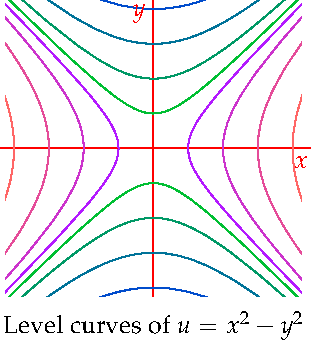
\includegraphics{functions-zsq}
	\end{minipage}
	\goodbreak
	
	%Away from the origin, $f(\pm z)=z^2$ shows that $f$ is a \emph{two-to-one} function.
	The polar form allows us to think about the what $f$ does to the argument:
	\[
		f(z)=r^2e^{2i\theta}\implies \arg f(z)=2\arg z
	\]
	Given a \textcolor{Green}{sector} between arguments $\theta$ and $\phi$, the function \emph{doubles} this to the \textcolor{blue}{sector} between $2\theta$ and $2\phi$. This can also be visualized pathwise. If $z$ traces a \textcolor{Green}{path} which once encircles the origin, then the \textcolor{blue}{path} traced by $z^2$ orbits the origin \emph{twice}. The colored dots on the two paths correspond under $\textcolor{Green}{z}\mapsto \textcolor{blue}{z^2}$.
	\begin{center}
		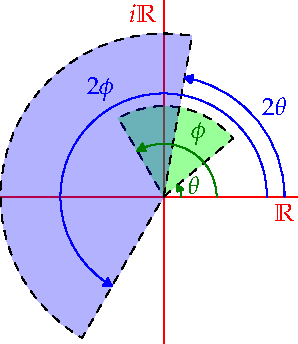
\includegraphics{functions-zsq2}
		\qquad\qquad
		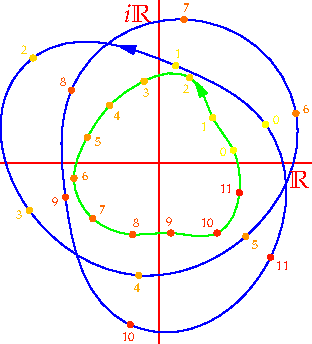
\includegraphics{functions-zsq3}
	\end{center}
\end{example}

	Similar behavior occurs with higher powers. For instance, $z\mapsto z^3$ maps a single loop round the origin to a \emph{triple} loop. %; away from the origin we have a \emph{three-to-one} function. 
	By contrast, the principal square root function $\sqrt z=\sqrt r\polar{i\theta}2$ \emph{halves} the principal argument: $\Arg\sqrt z\in (-\frac\pi 2,\frac\pi 2]$. In the fractional-exponent language of Section \ref{sec:roots},
	\[
		z\mapsto z^{1/2} =\{\sqrt r\polar{i\theta}2,-\sqrt r\polar{i\theta}2\}
	\]
	This is sometimes called a \emph{two-valued} function---we'll return to such objects in Chapter \ref{chap:functions}.


\boldsubsubsection{2D geometry with complex numbers}\phantomsection\label{pg:2dgeom}

Complex functions easily describe the basic geometric transformations of the plane.
\begin{description}
	\item[Translation] If $w$ is constant, the function $f(z)=z+w$ translates the plane, shifting the origin to $w$.
	\item[Scaling] If $R>0$ is a real constant, the function $f(z)=Rz$ scales/stretches the complex plane relative to the origin.
	\item[Rotation] Given $\phi\in\R$, the function $f(z)=e^{i\phi}z$ rotates the plane by $\phi$ radians counter-clockwise around the origin. This is easy to see in polar form:
	\[
		f(z)=f(re^{i\theta})=e^{i\phi}re^{i\theta}=re^{i(\theta+\phi)}
	\]
	\item[Reflection] Complex conjugation $f(z)=\cl z=x-iy$ reflects the plane in the horizontal axis.
\end{description}

By composing such functions, we can describe arbitrary rotations, reflections and scalings relative to any points/lines.



\begin{examples}{}{analyticpg2}
	\exstart We construct rotation by $\frac\pi 3=\ang{60}$ counter-clockwise about $2i$ in three stages:
	\begin{enumerate}\setcounter{enumi}{1}
	  \item[]\begin{enumerate}
	  	\item Translate $2i$ to the origin: \ $z\mapsto z-2i$
	  	\item Rotate by $\frac\pi 3$ about the origin: \ $z\mapsto e^{\frac{i\pi}3}(z-2i)$
	  	\item Translate the origin back to $2i$: \ $z\mapsto f(z) =\polar{i\pi}3(z-2i)+2i$
		\end{enumerate}
	  
		\item We may similarly produce any reflection. To reflect in the line through 0 and $w$ with $\Arg w=\phi$;
		\begin{enumerate}
		  \item Rotate the plane by $-\phi$: \ $z\mapsto e^{-i\phi}z$
		  \item Reflect in the real axis: \ $z\mapsto \cl{e^{-i\phi}z}=e^{i\phi}\cl z$
		  \item Rotate the plane back by $\phi$: \ $z\mapsto f(z)=e^{2i\phi}\cl z$
		\end{enumerate}
	  
	  \item\label{ex:reflect2} We compute the function that reflects across the line joining $\alpha=2+i$ and $\beta=4+3i$.\smallbreak
	  Since $\beta-\alpha=2+2i$ has argument $\phi=\frac\pi 4$, we combine reflection across the line making $\phi$ through the origin with translation by $\alpha$ (translate by $-\alpha$, reflect, translate back by $\alpha$):
	  \begin{align*}
		  f(z)&=e^{2i\phi}(\cl{z-\alpha})+\alpha =\polar{i\pi}2(\cl{z-2-i})+2+i=i(\cl z-2+i)+2+i\\
		  &=i\cl z+1-i
	  \end{align*}
	  As a sanity check, you should verify explicitly that $f(\alpha)=\alpha$ and $f(\beta)=\beta$: why?
	\end{enumerate}
\end{examples}


\begin{exercises}
	\exstart For each function, describe its implied domain (page \pageref{sec:func}).
	\begin{enumerate}\setcounter{enumi}{1}
	  \item[]\begin{enumerate}
	    \item $\displaystyle f(z)=\frac 1{4+z^2}$\qquad
	    (b) \ $\displaystyle f(z)=\frac{z-1}{e^z-1}$\qquad
	    (c) \ $\displaystyle f(z)=\frac{z^2+z+1}{z^4-1}$
	  \end{enumerate}
	  
	  
	  \item Write the function in terms of its real and imaginary parts: $f(z)=u(x,y)+iv(x,y)$.
	  \begin{enumerate}
	  	\item $\displaystyle f(z)=z^3-4z^2+2$\qquad
	    (b) \ $\displaystyle f(z)=\frac{z^2}{1-\cl z}$\qquad
	    (c) \ $\displaystyle f(z)=e^{\cl z}$
	  \end{enumerate}
	  
	  
	  \item Write the function $\displaystyle f(z)=\frac 1{\nm z^2}\cl z$ in polar form.
	  
	  
	  \item Find an expression for the function which reflects across the vertical line through $\alpha=-1$.
	  
	  
	  \item In Example \ref*{ex:analyticpg2}.\ref{ex:reflect2}, evaluate the function $\displaystyle g(z)=e^{2i\phi}(\cl{z-\beta})+\beta$. Why are you not surprised by the result?
	  
	  
	  \item Let $\phi=\tan^{-1}\frac 34$. Find the result (in rectangular co-ordinates) of rotating $z=-2+i$ counter-clockwise by $\phi$ radians around the origin.\par
	  (\emph{Hint: consider a 3:4:5 triangle!})
	  
	  
	  \item Prove, using the expressions on page \pageref{pg:2dgeom}, that the composition of two reflections is a rotation, and that the composition of a rotation and a reflection is a reflection.
	\end{enumerate}
\end{exercises}

\clearpage



\subsection{Open sets, Limits and Continuity}\label{sec:opensets}

This section is mostly for reference, since limits and continuity behave similarly to real analysis. Indeed proofs are often identical, so we mostly omit them. If you're only familiar with \emph{single-variable} real analysis, note particularly how the first definition generalizes the notion of an \emph{open interval}.


\begin{defn}{Disks and Neighborhoods}{disks}
	Given $\delta>0$ and $z_0\in\C$, the \emph{\textcolor{Green}{open disk}} (or \emph{$\delta$-ball}) centered at $z_0\in\C$ with radius $\delta$ is the set\par
	\begin{minipage}[t]{0.7\linewidth}\vspace{-15pt}
		\[
			B_\delta(z_0)=\{z\in\C:\nm{z-z_0}<\delta\}
		\]
		Remove the central point $z_0$ for the corresponding \emph{punctured open disk}:
		\[
			\{z\in\C:0<\nm{z-z_0}<\delta\}
		\]
		Now let $D\subseteq\C$ be a subset.
	\end{minipage}
	\hfill
	\begin{minipage}[t]{0.29\linewidth}\vspace{-16pt}
		\centering%
		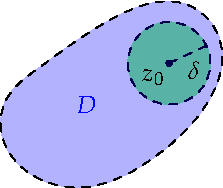
\includegraphics[scale=0.9]{functions-open}\\
		An \textcolor{blue}{open neighborhood} of $z_0$
	\end{minipage}
	\par\vspace{-5pt}
	\begin{itemize}\itemsep0pt
		\item $D$ is \emph{open} if every point is \emph{interior}: at every $z_0\in D$ we may center some open disk $B_\delta(z_0)\subseteq D$:\vspace{-2pt}
		\[
			\forall z_0\in D, \ \exists \delta>0\text{ such that } \nm{z-z_0}<\delta\implies z\in D
		\]\vspace{-20pt}
		\item $D$ is a \emph{neighborhood} of $z_0$ if it contains some $B_\delta(z_0)$. A neighborhood can, but need not, be open. A \emph{punctured neighborhood} instead contains a punctured disk.
		\item $D$ is \emph{closed} if its complement $\C\setminus D$ is open.
	\end{itemize}
\end{defn}

\begin{example}[lower separated=false, sidebyside, sidebyside align=top seam, sidebyside gap=0pt, righthand width=0.25\linewidth]{}{easyopen}
	The punctured plane $D=\C\setminus\{2+i\}$ is an open set. For instance, given $z_0\in D$, let $\delta=\frac 12\nm{z_0-2-i}$, then $\textcolor{Green}{B_\delta(z_0)}\subset D$.\par
	(The $\frac 12$ is superfluous, since the disk $B_\delta(z_0)$ does not contain its boundary, it just makes for a clearer picture.)
	\tcblower
	\flushright
	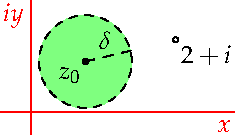
\includegraphics[scale=0.9]{limits-punctured}
\end{example}

\begin{defn}{Sequences and Limits}{}{}
	Let $(z_n)=(z_1,z_2,\ldots)$ be a \emph{sequence} of complex numbers.
	\begin{enumerate}\itemsep0pt
	  \item $(z_n)$ \emph{converges} to $z_0\in\C$, and we write \smash[b]{$\lim\limits_{n\to \infty}z_n=z_0$} or simply $z_n\to z_0$, if\vspace{-2pt}
		\[
			\forall \epsilon>0,\ \exists N\text{ such that }n>N\implies \nm{z_n-z_0}<\epsilon
		\]
		\vspace{-20pt}
		
		\item $(z_n)$ is a \emph{Cauchy sequence} if\vspace{-2pt}
		\[
			\forall \epsilon>0,\ \exists N\text{ such that }m,n>N\implies \nm{z_m-z_n}<\epsilon
		\]
	\end{enumerate}
\end{defn}


\begin{thm}{Useful Facts about Sequences}{compbolzano}
	\exstart $(z_n)$ is convergent/Cauchy if and only if its real and imaginary parts are also, as follows from two straightforward inequalities:
	\[
		%\max\{\nm{x_n-x_0},\nm{y_n-y_0} \} \le 
		\nm{z_n-z_0} \le \nm{x_n-x_0}+\nm{y_n-y_0} \le 2\nm{z_n-z_0}
	\]
	\begin{enumerate}\setcounter{enumi}{1}\itemsep1pt
	  \item Cauchy completeness: $(z_n)$ converges in $\C$ if and only if it is Cauchy
	  \item Bolzano--Weierstraß: If $(z_n)$ is bounded, then it has a convergent subsequence.
	  \item\label{thm:closedlimit3} $D\subseteq\C$ is closed if and only if every Cauchy sequence $(z_n)\subseteq D$ has its limit in $D$.
	\end{enumerate}
\end{thm}


\goodbreak


\begin{defn}{Continuity}{contdef}
	Let $f:D\to\C$ and $z_0\in D$. We say that $f$ is \emph{continuous at $z_0$} if
	\[
		\text{For all sequences } (z_n)\subseteq D\text{ with }\lim z_n=z_0\text{ we have }\lim f(z_n) = f(z_0)
	\]
	$f$ is \emph{continuous} (on $D$) if it is continuous at all points $z_0\in D$.
\end{defn}


Rather than using sequences, we'll typically consider continuity via limits of functions.

\begin{defn}{Limits of Functions}{limit}
	Let $f:D\to\C$, where $D$ contains an open punctured neighborhood of $z_0$. We say that $w_0$ is the \emph{limit of $f$ as $z$ approaches $z_0$}, written $\lim\limits_{z\to z_0}f(z)=w_0$, if
	\[
		\forall \epsilon>0,\ \exists \delta>0\text{ such that } 0<\nm{z-z_0}<\delta\implies \nm{f(z)-w_0}<\epsilon
	\]
\end{defn}

Otherwise said, given an $\epsilon$-ball centered at $w_0$, there is a $\delta$-ball $B_\delta(z_0)$ such that $f\bigl(B_\delta(z_0)\bigr)\subseteq B_\epsilon (w_0)$. Equivalently, $\forall (z_n)\subseteq D\setminus\{z_0\}$, $\lim z_n=z_0\Longrightarrow \lim f(z_n)=w_0$. This is almost continuity!

\begin{thm}{}{}
	Let $z_0$ be an \emph{interior} point of $D$. Then $f:D\to\C$ is continuous at $z_0$ if and only if
	\[
		\lim\limits_{z\to z_0}f(z)=f(z_0)
	\]
\end{thm}

% Otherwise said, for any $\epsilon$-ball $B_\epsilon\bigl(f(z_0)\bigr)$, there exists a $\delta$-ball $B_\delta(z_0)$ such that $f\bigl(B_\delta(z_0)\bigr)\subseteq B_\epsilon\bigl(f(z_0)\bigr)$.
\medbreak



\begin{example}{}{}
	Calculations tend to proceed similarly to real analysis. For instance, we show that $f(z)=z^2$ is continuous (on $\C$) by proving that $\lim\limits_{z\to z_0}z^2=z_0^2$ for all $z_0$.\smallbreak
	Let $z_0\in\C$ and $\epsilon>0$ be given. Define $\delta=\min\{1,\frac\epsilon{1+2\nm{z_0}}\}$. By the triangle-inequality,
	\begin{align*}
		\nm{z-z_0}<\delta&\implies \nm{z+z_0}=\nm{z-z_0+2z_0}\le \nm{z-z_0}+2\nm{z_0}<\delta+2\nm{z_0}\le 1+2\nm{z_0}\\
		&\implies \nm{z^2-z_0^2}=\nm{z-z_0}\nm{z+z_0}<\delta(1+2\nm{z_0})\le \epsilon
	\end{align*}
	The picture should help: given an \textcolor{blue}{$\epsilon$-ball} centered at $w_0=z_0^2$, we've described how to choose $\delta>0$ so that $f$ maps the \textcolor{Green}{$\delta$-ball} centered at $z_0$ to a \textcolor{Green}{region} \emph{inside} the original \textcolor{blue}{$\epsilon$-ball.}
	\begin{center}
		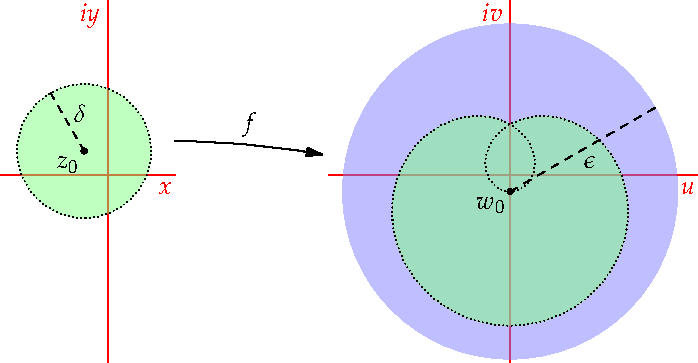
\includegraphics[scale=0.85]{limits-zsq}
	\end{center}
	The picture illustrates the case when
	\[
		z_0=\frac 12\polar{3\pi i}4=\frac 1{2\sqrt 2}(-1+i),\quad w_0=-\frac i4,\quad \epsilon=\frac 52\quad\text{and}\quad \delta=\min\left\{1,\tfrac{5/2}{1+2\cdot\frac 12}\right\}=1
	\]
\end{example}
\goodbreak


\begin{thm}{Basic Facts about Limits of Functions}{basiclimit}
Suppose $f,g:D\to\C$ are functions and $z_0=x_0+iy_0$ is a point satisfying the assumptions of Definition \ref{defn:limit}.
\begin{enumerate}
  \item Limits are unique: If $w_0$ and $\widetilde{w_0}$ satisfy Definition \ref{defn:limit}, then $\widetilde{w_0}=w_0$.
  \item\label{thmbaslim2} If $f(z)=u(x,y)+iv(x,y)$ and $w_0=u_0+iv_0$, then
  \[
  	\lim_{z\to z_0}f(z)=w_0\iff \lim_{(x,y)\to (x_0,y_0)}\hspace*{-10pt} u(x,y)=u_0\quad \text{and}\quad \lim_{(x,y)\to (x_0,y_0)}\hspace*{-10pt} v(x,y)=v_0
  \]
  In particular $\lim\limits_{z\to z_0}\cl z=\cl{z_0}$
  \item Suppose $\lim\limits_{z\to z_0}f(z)=w_0$ and $\lim\limits_{z\to z_0}g(z)=w_1$:
  \begin{enumerate}
    \item For any $a,b\in\C$, $\lim\limits_{z\to z_0}\bigl( af(z)+bg(z)\bigr)=aw_0+bw_1$
    \item $\lim\limits_{z\to z_0}\bigl(f(z)g(z)\bigr)=w_0w_1$
    \item $\lim\limits_{z\to z_0}\frac{f(z)}{g(z)}=\frac{w_0}{w_1}$, provided $w_1\neq 0$ and $g(z)\neq 0$ on a punctured neighbourhood of $z_0$.
    \item If $h$ is a function such that $\lim\limits_{w\to w_0}h(w)=w_2$, then $\lim\limits_{z\to z_0}h(f(z))=w_2$
	\end{enumerate}
\end{enumerate}
\end{thm}

The basic limit laws should feel familiar and intuitive; indeed analogues of most should have been proved in real analysis. Parts 2 \& 3 have obvious corollaries for continuous functions. For instance:

\begin{cor}{}{}
	$f:D\subseteq\C\to\C$ is continuous if and only if its real and imaginary parts $u,v:D\to\R$ are also continuous. 
\end{cor}

Several pieces of part 3 follow from part 2 by considering real and imaginary parts and the limit laws for functions $\R^2\to\R$. For instance, write $f(z)=u_1+iv_1$ and $g(z)=u_2+iv_2$, then
\[
	\lim\limits_{z\to z_0}\bigl(f(z)g(z)\bigr) =\lim\limits_{z\to z_0}\bigl(u_1u_2-v_1v_2+i(u_1v_2+v_1u_2)\bigr) =w_0w_1
\]

\begin{examples}{}{}
	\exstart $\lim\limits_{z\to 1+3i}(z^2-i\cl z) =(1+3i)^2-i\bigl(\cl{1+3i}\bigr) =1+6i-9-i(1-3i)=-11+5i$.
	\begin{enumerate}\setcounter{enumi}{1}
	  \item Every polynomial function is continuous on $\C$.
	  \item Every rational function $f(z)=\frac{p(z)}{q(z)}$ (where $p,q$ are polynomials), is continuous on its implied domain $D=\{z:q(z)\neq 0\}$.
	  \item The exponential function
	  \[
	  	\exp(z)=e^z=e^xe^{iy}=e^x\cos y+ie^x\sin y
	  \]
	  is continuous on $\C$, since the exponential, cosine and sine are continuous on $\R$.
	\end{enumerate}
\end{examples}

\vfil\goodbreak


\boldsubsubsection{Limits and the Point at Infinity}

In (single-variable) real analysis there are \emph{two} infinities ($\pm\infty$). In complex analysis, the convention is to have only one: for instance, the sequences $z_n=n$ and $w_n=in$ both diverge to the \emph{same} infinity.

\begin{defn}{}{rsphere}
	The \emph{extended complex plane} (\emph{Riemann sphere}) is the set $\cl\C=\C\cup\{\infty\}$ where $\infty$ denotes the \emph{point at infinity.} The concepts of \emph{neighborhood, openness} and \emph{limit} extend naturally:\vspace{-3pt}
	\begin{enumerate}\itemsep0pt
	  \item A \emph{neighborhood} of $\infty$ is any set containing an \emph{open disk} at $\infty$, namely a subset of the form\vspace{-3pt}
		\[
			\{\infty\}\cup\{z\in\C:\nm{z}>M\}
		\]
	  \item\vspace{-5pt} $\lim\limits_{z\to z_0}f(z)=\infty$ means: $\forall M>0$, $\exists \delta>0$ such that $0<\nm{z-z_0}<\delta \implies \nm{f(z)}>M$
	  \item $\lim\limits_{z\to \infty}f(z)=w_0$ means: $\forall \epsilon>0$, $\exists N>0$ such that $\nm{z}>N \implies \nm{f(z)-w_0}<\epsilon$
	  \item $\lim\limits_{z\to\infty}f(z)=\infty$ means: $\forall M>0$, $\exists N>0$ such that $\nm{z}>N\implies \nm{f(z)}>M$
	\end{enumerate}
\end{defn}

These limits have the same interpretation as Definition \ref{defn:limit}: `$z$ close to $z_0$' implies `$f(z)$ close to $w_0$.' The difficulty is merely about the meaning of `close to $\infty$' when $z_0$ or $w_0$ is the point at infinity. 

\begin{example}{}{}
	We verify that $\smash{\lim\limits_{z\to -3i}}\,\frac{z^2}{z+3i}=\infty$. Let $M>0$ be given and define $\delta=\min\{1,\frac 4{M}\}$. Then
  \[
  	0<\nm{z+3i}<\delta \implies \nm z\overset{\triangle}{\ge} \nm{3i}-\nm{z+3i}>3-\delta\ge 2 \implies \nm{\frac{z^2}{z+3i}} > \frac{4}{\delta} \ge M
  \]
\end{example}


The relationship between limits, zero and infinity feel like the dubious claims $\frac 1\infty=0$ and $\frac 10=\infty$!

\begin{thm}{}{infty}
	Provided all limits make sense, Theorem \ref{thm:basiclimit} also applies to limits involving infinity. Moreover, we have the additional relationships:
	\begin{enumerate}
	  \item $\lim\limits_{z\to z_0}f(z)=\infty \iff \lim\limits_{z\to z_0}\frac 1{f(z)}=0$ \qquad\qquad 2.\ \ $\lim\limits_{z\to\infty}f(z)=w_0 \iff \lim\limits_{\zeta\to 0}f\left(\frac 1{\zeta}\right)=w_0$
	  \setcounter{enumi}{2}
	  \item $\lim\limits_{z\to \infty}f(z)=\infty \iff \lim\limits_{\zeta\to 0}\frac 1{f(1/\zeta)}=0$
	\end{enumerate}
\end{thm}

\begin{proof}[Sketch Proof]
	All six results are similar; we prove only the $\Rightarrow$ direction of the second. Suppose $\epsilon>0$ is given. Then $N$ exists according to Definition \ref{defn:rsphere} (part 3). Let $\delta=\frac 1N$ and $\zeta=\frac 1z$, then
	\[
		0< \nm \zeta<\delta 
		\implies \nm z =\tfrac 1{\nm\zeta}>N
		\implies \nm{f(\tfrac 1\zeta)-w_0}=\nm{f(z)-w_0}<\epsilon \tag*{\qedhere}
	\]
\end{proof}


\begin{example}{}{}
	Consider $f(z)=\frac{5iz+1}{3z-2i}$. Plainly 
  \begin{gather*}
  	\lim_{z\to\frac 23i}\frac 1{f(z)}
  	=\lim_{z\to\frac 23i}\frac{3z-2i}{5iz+1}=0
  	\implies \lim_{z\to\frac 23i}f(z)=\infty
  	,\qquad
  	\lim_{z\to\infty}f(z)%= \lim_{z\to\infty}\frac{5i+\frac 1z}{3-\frac{2i}z} 
  	=\frac{5i+\lim\frac 1z}{3-2i\lim\frac 1z}
  	=\frac 53i
  \end{gather*}
	Because of this, it is common to view $f$ as a continuous bijection $f:\cl\C\to\cl\C$ (exercise):
% \[
% 	f(z):=
% 	\begin{cases}
% 		\frac{5iz+1}{3z-2i}&\text{if }z\neq \frac 23i,\infty\\
% 		\infty&\text{if }z=\frac 23i\\
% 		\frac 53i&\text{if }z=\infty
% 	\end{cases}
% \]
\[
	f(z)=\frac{5iz+1}{3z-2i}\quad \bigl(\text{if }z\neq \tfrac 23i,\infty\bigr),\qquad f\left(\frac 23i\right)=\infty,\qquad f(\infty)=\frac 53i
\]
\end{example}

\goodbreak


\begin{aside}{\bf Aside (non-examinable)}{}
	The Riemann sphere is merely a fun diversion for us. Unless indicated otherwise, all sets should be assumed to be subsets of the (\emph{finite}) complex plane.\par
	\begin{minipage}[t]{0.54\linewidth}\vspace{-5pt}
		The Riemann sphere can be visualized as a \textcolor{blue}{sphere $S^2$}, with $\infty$ playing the role of the north pole. The rest of the sphere is identified bijectively with the \textcolor{Green}{equatorial plane $\C$} via \href{https://en.wikipedia.org/wiki/Stereographic_projection}{\emph{stereographic projection}} $\pi:S^2\to\cl\C$. In the picture, the image of $P\in S^2$ is the intersection $\pi(P)$ of $\C$ with the line through $P$ and $N=\pi^{-1}(\infty)$.
	\end{minipage}
	\hfill
	\begin{minipage}[t]{0.45\linewidth}\vspace{-4pt}
		\flushright%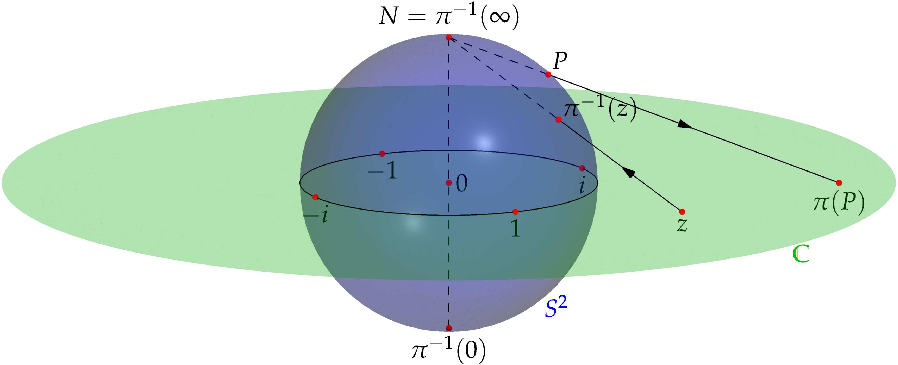
\includegraphics{complex-stereo+0_0}
		\href{https://www.math.uci.edu/~ndonalds/math147/complex-stereo.html}{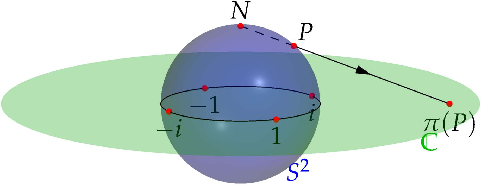
\includegraphics[scale=0.9]{complex-stereo}}
	\end{minipage}
\end{aside}

 
\boldsubsubsection{Compactness, Path-Connectedness \& Continuity}

We finish with two further desirable properties of domains.

\begin{defn}{}{}
	\exstart A subset $K\subseteq\C$ is \emph{compact} if it is closed and bounded.
	\begin{enumerate}\setcounter{enumi}{1}
	  \begin{minipage}[t]{0.61\linewidth}\vspace{-5pt}
	  	\item $K\subseteq\C$ is \emph{(path-)connected}\footnotemark{} if any two points can be joined by a path lying within $K$: more precisely, $\forall p,q\in K$,
	  	\[
	  		\exists z:[0,1]\to K \text{ continuous } \text{ with }
	  z(0)=p \text{ and }z(1)=q
	  	\]
	  \end{minipage}
	  \hfill 
	  \begin{minipage}[t]{0.38\linewidth}\vspace{-20pt}
			\flushright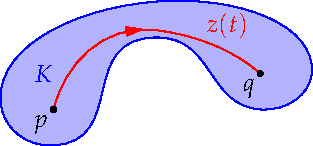
\includegraphics{limits-topology}
	  \end{minipage} 
	\end{enumerate} 
\end{defn}

\footnotetext{%
	Loosely speaking, a connected set consists of one `lump.' If you've studied topology: almost all domains in these notes will be open, so there is no benefit to distinguishing between connectedness and path-connectedness.
}


These concepts generalize notions of intervals from single-variable real analysis. In view of this, we translate two familiar results, essentially the \emph{extreme} and \emph{intermediate value theorems} of real analysis.

\begin{thm}{}{compactconnected}
	Suppose $f:K\to\C$ is continuous.
	\begin{enumerate}
  	\item If $K$ is compact, so is the image $f(K)$.
  	\item If $K$ is path-connected, so is $f(K)$.
	\end{enumerate}
\end{thm}

\begin{proof}{}{}
	\begin{enumerate}
	  \item Consider the \emph{real-valued} function $\nm{f}$ and apply the same argument from real analysis:
		\begin{itemize}%\itemsep0pt
		  \item Let $M=\sup\{\nm{f(z)}:z\in K\}$. Then $\exists (z_n)\subseteq K$ such that $\lim\nm{f(z_n)} =M$.
		  \item $K$ is bounded; Bolzano--Weierstraß says $(z_n)$ has a convergent subsequence $(z_{n_k})$.
		  \item Let $z_0=\lim z_{n_k}$. Since $K$ is closed we have $z_0\in K$ (Theorem \ref*{thm:compbolzano}.\ref{thm:closedlimit3}), whence $f(z_0)$ is defined.
		  \item $f$ continuous $\Longrightarrow\lim f(z_{n_k})= f(z_0)$; thus $M=f(z_0)$ is finite and $f(K)$ is bounded.
		  \item The closure of $f(K)$ is a short exercise.
		\end{itemize}
		\item This is also an exercise.\qedhere
	\end{enumerate}
\end{proof}


% Later on we'll need one final fact about compactness, which we again state without proof.
% 
% \begin{thm}{}{opencover}
% 	Let $K$ be compact and suppose that a collection of open sets $U_j$ satisfies $K\subseteq \smash[b]{\bigcup\limits_{j\in I} U_j}$.\par
% 	Then there exists a \textbf{finite} subset $J\subseteq I$ such that $K\subseteq \bigcup\limits_{j\in J} U_j$.
% \end{thm}
% 
% This is usually said ``Every open cover has a finite subcover,'' and is taken, in topology, as the definition of compactness. That this is equivalent to being closed and bounded in $\C$ (or any Euclidean space) is the famous Heine--Borel Theorem.\smallbreak

The upshot of this section is that continuity and limits are essentially the same in both real and complex analysis and behave as you should expect. Differentiation, however, is another beast entirely\ldots

\vfil\vfil\clearpage


\begin{exercises}{}{}
	\exstart As in Example \ref{ex:easyopen}, prove that the doubly-punctured plane $D:=\C\setminus\{1,-2i\}$ is an open set. State a function whose implied domain is this set.\vspace{-2pt}

	\begin{enumerate}\setcounter{enumi}{1}
	  \item Use the $\epsilon$--$\delta$ definition (\ref{defn:limit}) to prove the following.\vspace{-2pt}
	  \begin{enumerate}
	  	\item $\displaystyle\lim\limits_{z\to z_0}\cl z=\cl{z_0}$\qquad
	  	(b) \ $\displaystyle\lim\limits_{z\to 0}\frac{\cl z^2}z=0$\qquad
	  	(c) \ $\displaystyle\lim\limits_{z\to 2}\frac 1{z-i}=\frac 1{2-i}$\qquad
	  	(d) \ $\displaystyle\lim\limits_{z\to z_0}z^3=z_0^3$
	  \end{enumerate}
	  
	  
	  \item Show that $f(z)=(z/\cl z)^2$ equals 1 at all non-zero points on the real and imaginary axes, and $-1$ at all non-zero points on the line $y=x$. Explain why \smash{$\lim\limits_{z\to 0}f(z)$} doesn't exist.
	  
	  
	  \item Prove part 3(c) of Theorem \ref{thm:basiclimit}.
	  
	  
	  \item Suppose \smash{$\lim\limits_{z\to z_0}f(z)=w_0$}. Prove that \smash{$\lim\limits_{z\to z_0}\nm{f(z)}=\nm{w_0}$.}
	   
	   
	  \item Use Definition \ref{defn:rsphere} to prove part of Theorem \ref{thm:infty}: \smash{$\lim\limits_{z\to z_0}f(z)=\infty \implies \lim\limits_{z\to z_0}\frac 1{f(z)}=0$.}
	  
	  
	  \item Use Definition \ref{defn:rsphere} to prove: (a)\lstsp \smash{$\lim\limits_{z\to 2i}\frac{iz-1}{z-2i}=\infty$, 
	    \qquad (b) \ $\lim\limits_{z\to\infty}\frac{iz-1}{z-2i}=i$}
% 	  \begin{enumerate}
% 	    \item $\displaystyle\lim\limits_{z\to 2i}\frac{iz-1}{z-2i}=\infty$ 
% 	    \qquad (b) \ $\displaystyle\lim\limits_{z\to\infty}\frac{iz-1}{z-2i}=i$
% 	  \end{enumerate}
	  
	  
	 	\item\begin{enumerate}
	    \item Show that $f(z)=\frac{5iz+1}{3z-2i}$ defines a bijection of the Riemann sphere $f:\cl\C\to\cl\C$.\par
	  	(\emph{Hint: let $w=f(z)$ and solve for $z\ldots$})
	  	
	  	\item In general: Given $\alpha,\beta,\gamma,\delta\in\C$, prove that $f(z)=\frac{\alpha z+\beta}{\gamma z+\delta}$ defines a bijection of the Riemann sphere if and only if $\alpha\delta-\beta\gamma\neq 0$. How does this relate to the matrix
	  	$\smash{
	  		\begin{smatrix}
	  			\alpha&\beta\\
	  			\gamma&\delta
	  		\end{smatrix}
	  	}$?
	  \end{enumerate}
	  
	  
	  \item We complete the proof of Theorem \ref{thm:compactconnected}. Suppose $f:K\subseteq\C\to\C$ is continuous.
	  \begin{enumerate}
	    \item Let $K$ be compact. Suppose $(w_n)\subseteq K$ is a sequence where $\bigl(f(w_n)\bigr)$ is convergent in $\C$. Explain why there exists a convergent subsequence $(w_{n_k})$, and use it to show that $\lim f(w_n)\in f(K)$. Hence conclude that $f(K)$ is closed.
	    
			\item Suppose $K$ is path-connected. If $f(p),f(q)\in f(K)$, show that $\exists w:[0,1]\to f(K)$ continuous such that $w(0)=f(p)$ and $w(1)=f(q)$. Hence conclude that $f(K)$ is path-connected.
	  \end{enumerate}
	  
	  
	  \item\label{exs:finitesubcover} (Hard)\lstsp ``Every open cover has a finite subcover,'' is a crucial result in topology:\footnotemark{}
	  \begin{quote}
	  	\textbf{Theorem}\lstsp Suppose a compact $K$ is a subset of a (possibly infinite) union $\bigcup U_j$ of open sets. Then there are \emph{finitely} many $U_j$ (labelled WLOG) such that $K\subset U_1\cup\cdots\cup U_n$.
	  \end{quote}
	  Suppose $z:[0,1]\to D\subseteq\C$ is a \textcolor{red}{path} in an open domain $D$ and define $K=\operatorname{range}{z}$.
		\begin{enumerate}
	  	\begin{minipage}[t]{0.66\linewidth}\vspace{-4pt}
	    	\item Explain why $K$ is compact.
	    	\item Prove that $K$ may be covered by \emph{finitely} many \emph{closed} balls $\cl{B_k}$ for which $K\subset B_0\cup\cdots\cup B_n\subset\cl{B_0}\cup\cdots\cup\cl{B_n}\subset D$.\par
	      (\emph{Hint: start by centering a ball at \textbf{every} point of $K$})
	      \item Prove that $D$ contains a \textcolor{purple}{zig-zag path} (finitely many horizontal/vertical segments) from $z(0)$ to $z(1)$.
			\end{minipage}
			\hfill
			\begin{minipage}[t]{0.33\linewidth}\vspace{-10pt}
				\flushright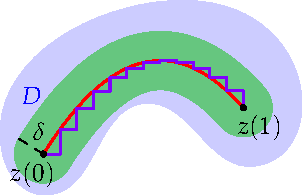
\includegraphics[scale=0.95]{analytic-topology4}
			\end{minipage}\par
			\item Show that we can fit a `\textcolor{Green}{tube}' around $K$: $\exists\delta>0$ such that $\forall z\in K,\ \nm{z-w}\le\delta\Longrightarrow w\in D$.\par
			(\emph{Hint: following part (b), let $V=\bigcup\cl{B_k}\setminus\bigcup B_k$ and define $\delta:=\inf\bigl\{\nm{z-v}:z\in K,v\in V\bigr\}$})
		\end{enumerate}
		
	\end{enumerate}
\end{exercises}

\vspace{-10pt}

\footnotetext{%
	This is often taken as the definition of compactness in topology. Its equivalence to $K$ being closed and bounded in $\C$ (or any Euclidean space) is the famous Heine--Borel Theorem.
}

\clearpage



\subsection[Derivatives \& Cauchy--Riemann]{Derivatives \& the Cauchy--Riemann Equations}% (\S\,19-23)

Differentiation is where complex analysis starts to produce interesting and novel results. It won't appear so initially, since the definition of derivative is exactly as you've previously encountered.

\begin{defn}{}{deriv}
	Let $f:D\to\C$ be a complex function and $z_0$ an \emph{interior} point of $D$. We say that $f$ is \emph{differentiable at $z_0$} if the following limit exists:
	\[
		\lim_{z\to z_0}\frac{f(z)-f(z_0)}{z-z_0}
	\]
	We call this limit the \emph{derivative} of $f$ at $z_0$ and denote it $f'(z_0)$. If $f$ is differentiable everywhere\footnotemark{} on $D$ then the derivative is itself a function, written $f'(z)$ or $\diff[f]{z}$. 
\end{defn}

\footnotetext{Such \emph{holomorphic} functions are the main topic of the course: we'll consider them more properly in the next section. Necessarily, $D$ must be an open set if $f$ is to be holomorphic (think about the definition of the limit!).}


\begin{example}{}{}
	The function $f(z)=z^2$ is everywhere differentiable,
  \[
  	\lim_{z\to z_0}\frac{f(z)-f(z_0)}{z-z_0} =\lim_{z\to z_0}\frac{z^2-z_0^2}{z-z_0} =\lim_{z\to z_0}\frac{(z-z_0)(z+z_0)}{z-z_0} \mathrel{\textcolor{red}{=}} \lim_{z\to z_0}(z+z_0) =2z_0
  \]
	The \textcolor{red}{second last} equality follows since we only compute on the punctured disk $0<\nm{z-z_0}<\delta$ when taking limits (Definition \ref{defn:rsphere}).
\end{example}


The basic rules of differentiation are identical those in real analysis and can be proved similarly.

\begin{thm}{}{derivrules}
	Suppose $f$ and $g$ are differentiable (either at a point $z_0$ or as functions).
	\begin{enumerate}
	  \item (Linearity)\quad For any constants $a,b\in\C$, $\displaystyle\diff z\bigl(af(z)+bg(z)\bigr)=af'(z)+bg'(z)$
	  \item (Power Law)\quad For any $n\in\N_0$, $\displaystyle\diff zz^n=nz^{n-1}$
	  \item (Product rule)\quad $\displaystyle\diff z\bigl(f(z)g(z)\bigr)=f'(z)g(z)+f(z)g'(z)$
	  \item (Quotient Rule)\quad If $g(z)\neq 0$, then $\displaystyle\diff z\frac{f(z)}{g(z)}=\frac{f'(z)g(z)-f(z)g'(z)}{[g(z)]^2}$
	  \item (Chain Rule)\quad If $h$ is differentiable at $g(z_0)$, then $h\circ g$ is differentiable at $z_0$ and
	  \[
	  	(h\circ g)'(z_0)=h'\bigl(g(z_0)\bigr)g'(z_0)
	  \]
	\end{enumerate}
\end{thm}

We immediately see that all polynomials and rational functions are differentiable. Familiar examples behave the same regardless of whether we are in $\R$ or $\C$!

\begin{example}{}{}
  $\displaystyle\diff z\frac{3(z^2-2)^5+z^2}{z^3+1} = \frac{[30z(z^2-2)^4+2z)](z^3+1) -3z^2[3(z^2-2)^5+z^2]}{(z^3+1)^2}$
\end{example}


\vfil\goodbreak

\boldsubsubsection{The Cauchy--Riemann Equations}


Differentiation thus far seems uncontroversial; here is an example that might change your mind\ldots

\begin{example}{}{crconj}
	Consider  $f(z)=\cl z$ at a generic point $z_0=x_0+iy_0$, and the difference quotient
  \[
   	\frac{f(z)-f(z_0)}{z-z_0}=  \frac{x-iy-x_0+iy_0}{x+iy-x_0-iy_0} = \frac{\Delta x-i\Delta y}{\Delta x+i\Delta y} \tag{where $\Delta x=x-x_0$ and $\Delta y=y-y_0$}
  \]
  \begin{minipage}[t]{0.7\linewidth}\vspace{0pt}
	  For $f'(z)$ to exist, we must obtain the same limit \emph{regardless of how $(\Delta x,\Delta y)\to (0,0)$} (equivalent to $z\to z_0$). There are two obvious ways to take the limit:
	  \begin{itemize}
		  \item[]\normalfont\emph{\textcolor{blue}{Horizontally}}\quad $\displaystyle \frac{f(z)-f(z_0)}{z-z_0} =\frac{\Delta x}{\Delta x}=1$
		  \item[]\normalfont\emph{\textcolor{Green}{Vertically}}\quad $\displaystyle\frac{f(z)-f(z_0)}{z-z_0} =\frac{-i\Delta y}{i\Delta y}=-1$
	  \end{itemize}
  \end{minipage}
  \hfill
  \begin{minipage}[t]{0.29\linewidth}\vspace{-15pt}
  \flushright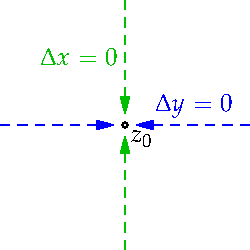
\includegraphics{diff-cr}  
  \end{minipage}
  \smallbreak
  The quotient plainly takes different values depending on how $(\Delta x,\Delta y)\to(0,0)$. We conclude that $f'(z_0)$ \emph{does not exist,} and that the function $f(z)=\cl z$ is \emph{nowhere differentiable}!
\end{example}

The approach extends to general functions. We attempt to differentiate $f(z)=u(x,y)+iv(x,y)$ (written in real and imaginary parts) at a generic point $z_0=x_0+iy_0$:
\[
	\lim\limits_{z\to z_0}\frac{f(z)-f(z_0)}{z-z_0}= \lim\limits_{(\Delta x,\Delta y)\to (0,0)}\frac{u(x,y)-u(x_0,y_0)+i(v(x,y)-v(x_0,y_0)}{\Delta x+i\Delta y}
\]
\emph{If this limit exists,} the same result must be obtained when evaluating along paths approaching $z_0$ horizontally and vertically. This results in a key relationship between the partial derivatives of $u,v$.
\begin{description}
	\item[\normalfont\emph{\textcolor{blue}{Horizontally}}]\quad We have $\Delta y=0$ ($y=y_0$), so the limit becomes
	\[
		\lim_{\Delta x\to 0} \frac{u(x,y_0)-u(x_0,y_0)+i(v(x,y_0)-v(x_0,y_0)}{\Delta x} =\left(\partials[u]{x}+i\partials[v]{x}\right)(x_0,y_0)
	\]
	\item[\normalfont\emph{\textcolor{Green}{Vertically}}]\quad We have $\Delta x=0$ ($x=x_0$), from which
	\[
		\lim_{\Delta y\to 0} \frac{u(x_0,y)-u(x_0,y_0)+i(v(x_0,y)-v(x_0,y_0)}{i\Delta y} =\frac 1i\left(\partials[u]{y}+i\partials[v]{y}\right)(x_0,y_0)
	\]
\end{description}

\begin{thm}{Cauchy--Riemann equations}{cauchyriemann}
	Write $f(z)=u+iv$ in its real and imaginary parts.
	\begin{enumerate}
	  \item If $f$ is complex-differentiable at $z_0$, then $u,v$ satisfy the \emph{Cauchy--Riemann equations} at $z_0$:
		\[
			\partials[u]{x}=\partials[v]{y} \quad\text{and}\quad \partials[u]{y}=-\partials[v]{x} \tag{equivalently $u_x=v_y$ and $u_y=-v_x$}
		\]
	  \item Conversely, if $u,v$ have partial derivatives on a neighborhood of $z_0$, which are continuous and satisfy the Cauchy--Riemann equations at $z_0$, then $f$ is complex-differentiable at $z_0$.
	\end{enumerate}
	In either situation, we may write $f'(z)=u_x+iv_x =v_y-iu_y$.
\end{thm}
We proved part 1 above. For a sketch of the almost-converse (part 2), see Exercise \ref{exs:crconv}.

%These aren't quite converses. For instance it is possible for a complex function to be differentiable at a single point but $u,v$ not to have cont partials there.

\goodbreak


\begin{examples}{}{crlots}
\exstart (Example \ref{ex:crconj})\lstsp $f(z)=\cl z=x-iy$ has $u(x,y)=x$ and $v(x,y)=-y$, whence
  \[
  	u_x=1\neq -1=v_y \quad\text{and}\quad u_y=0=v_x
  \]
  Since $u,v$ do not satisfy the Cauchy--Riemann equations, $f$ fails to be differentiable anywhere.
  
	\begin{enumerate}\setcounter{enumi}{1}
	  \item\label{exs:modnotdiff} $f(z)=\nm z=\sqrt{x^2+y^2}$ has $u=\sqrt{x^2+y^2}$ and $v=0$. Away from $z_0=0$, the Cauchy--Riemann equations are
	  \[
	  	u_x=\frac{x}{\sqrt{x^2+y^2}}=0=v_y,\quad u_y=\frac{y}{\sqrt{x^2+y^2}}=0=-v_x
	  \]
	  These equations are satisfied nowhere ($u,v$ are not differentiable at $z_0=0$), whence $f(z)$ is nowhere differentiable.
	  
	  \item $f(z)=z^2=x^2-y^2+2ixy$ has $u(x,y)=x^2-y^2$ and $v(x,y)=2xy$. We check
	  \[
	  	u_x=2x=v_y,\qquad u_y=-2y=-v_x
	  \]
	  As expected, $u,v$ satisfy the Cauchy--Riemann equations. Moreover,
	  \[
	  	f'(z)=2z=2x+2iy =u_x+iv_x =v_y-iu_y
	  \]
	  
	  \item\label{ex:cr3} Consider $\displaystyle f(z)=\frac z{2+\nm z^2}=\frac x{2+x^2+y^2}+\frac{iy}{2+x^2+y^2}$. We compute
	  \begin{gather*}
	  	u_x=\frac{2-x^2+y^2}{(2+x^2+y^2)^2} \qquad v_y=\frac{2+x^2-y^2}{(2+x^2+y^2)^2}\\
	  	u_y=\frac{-2xy}{(2+x^2+y^2)^2} \qquad -v_x=\frac{2xy}{(2+x^2+y^2)^2}
	  \end{gather*}
	  The Cauchy--Riemann equations are satisfied if and only if $xy=0=x^2-y^2$, which is if and only if $x=y=0$. We conclude that $f$ is not differentiable at any non-zero $z\in\C$.\smallbreak
	  Since the partial derivatives of $u,v$ are continuous, the converse of the Cauchy--Riemann theorem says that $f$ is differentiable at $z=0$: indeed
  	\[
  		f'(0)=u_x(0,0)+iv_x(0,0)=\frac 12
  	\]
	  We can alternatively check that this straight from the definition of derivative:
	  \[f'(0)=\lim_{z\to 0}\frac{f(z)-f(0)}{z-0}=\lim_{z\to 0}\frac 1{2+\nm z^2}=\frac 12\]
	  The function $f$ is therefore differentiable at precisely one point.
	  
		\item\label{ex:crexex2} The complex exponential function is everywhere differentiable: indeed
  	\[
  		f(z)=e^z=e^x\cos y+ie^x\sin y
  	\]
  	satisfies
  	\[
  		u_x=e^x\cos y=v_y,\qquad u_y=-e^x\sin x=-v_x
  	\]
  	where these are certainly continuous on $\C$. As expected,
  	\[
  		f'(z)=u_x+iv_x=e^x\cos y+ie^x\sin y =e^z
  	\]
	\end{enumerate}
\end{examples}

\goodbreak


\begin{exercises}{}
	\exstart Use Theorem \ref{thm:derivrules} to find the derivatives of the following functions:
	\begin{enumerate}\setcounter{enumi}{1}
	  \item[]\begin{enumerate}
	  	\item $\displaystyle f(z)=\frac 1{z^2+2z}$\qquad
	    (b) \ $\displaystyle f(z)=(z^3+2iz+1)^7$\qquad
	    (c) \ $\displaystyle f(z)=\frac{(3z^2-i)^3}{(iz^3+4)^2}$
	  \end{enumerate}
	  
	  
	  \item Use the limit definition of the derivative to compute the derivative of the functions:
	  \begin{enumerate}
	  	\item $\displaystyle f(z)=3z^3-iz^2$\qquad
	    (b) \ $\displaystyle f(z)=\frac 1{z^2}$
	  \end{enumerate}
	  
	  
	  \item Give a proof of the quotient rule, directly using the definition of the derivative.
	  
	  
	  \item Use the quotient rule to prove the power law for negative integer exponents:
	  \[
	  	\forall n\in\N,\quad \diff zz^{-n}=-nz^{-n-1}
	  \]
	  
	  
	  \item (\emph{L'Hôpital's rule})\lstsp Suppose $f(z_0)=g(z_0)=0$, and that $f'(z_0)$ and $g'(z_0)\neq 0$ both exist. Use the definition of the derivative to prove that
	  \[
	  	\lim_{z\to z_0}\frac{f(z)}{g(z)}=\frac{f'(z_0)}{g'(z_0)}
	  \]
	  
	  
	  \item Prove that $f(z)=\Re z$ and $g(z)=\Im z$ are not differentiable anywhere.
	  
	  
	  \item By writing $z=re^{i\theta}$ in polar form, verify directly that $f(z)=\nm z=\sqrt{x^2+y^2}$ is not differentiable at $z_0=0$.
	  
	  
	  \item What, if anything, do the Cauchy--Riemann equations allow you to conclude for the following?
	  \begin{enumerate}
	  	\item $\displaystyle f(z)=(z+i)^2$\qquad 
	  	(b) \ $\displaystyle f(z)= \frac{1}{\cl z-i}$\qquad
	    (c) \ $\displaystyle f(z)=z^3-\frac 2z$\qquad
	    (d) \ $\displaystyle f(z)=\bigl(\nm z^2+z\bigr)^2$
	  \end{enumerate}
	  
	  
	  \item As in Example \ref*{ex:crlots}.\ref{ex:crexex2}, prove that $\displaystyle \diff ze^{kz} =ke^{kz}$ for any complex constant $k=a+ib$.
	  
	  
	  \item Write a complex function $f(z)=f(z,\cl z)$ as a function of $z$ and $\cl z$. For example,
	  \[
	  	f(z)=\nm z^2=z\cl z
	  \]
	  Noting that $\displaystyle x=\frac 12(z+\cl z)$ and $\displaystyle y=\frac 1{2i}(z-\cl z)$, use the chain rule
	  \[
			\partials[f]{\cl z}=\partials[f]{x}\partials[x]{\cl z}+\partials[f]{y}\partials[y]{\cl z}
		\]
	  to prove that $f$ satisfies the Cauchy--Riemann equations if and only if $\displaystyle \partials[f]{\cl z}=0$.\smallbreak
	  Hence give a quick proof that $f(z)=z\cl z^2$ is not differentiable when $z\neq 0$.
	  
	  
	  \item\label{exs:crconv} Suppose $f(z)=u+iv$ satisfies the Cauchy--Riemann equations at $z_0=x_0+iy_0$. Use the multi-variable linear approximation
	  \[
	  	f(z)\approx f(z_0)+f_x(x_0,y_0)\Delta x+f_y(x_0,y_0)\Delta y
	  \]
	  to prove that $\frac{f(z)-f(z_0)}{z-z_0}\approx u_x(x_0,y_0)+iv_x(x_0,y_0)$ whenever $z\neq z_0$.\par
		(The existence/continuity assumptions in Theorem \ref{thm:cauchyriemann}, part 2, guarantee that this approximation becomes equality in the limit, though a rigorous proof requires more work)
	\end{enumerate}
\end{exercises}

\clearpage



\subsection[Holomorphic Functions]{Holomorphic and Harmonic Functions}\label{subsec:analytic}% (\S\,24--28)

We tend to be most interested in functions which are everywhere differentiable.

\begin{defn}{}{}
	We say that $f:D\to\C$ is:
	\begin{itemize}
	  \item \emph{Holomorphic} (or \emph{analytic}\footnotemark) on $D$ if it is differentiable at all points $z_0\in D$ (necessarily $D$ is open!).
	  \item \emph{Holomorphic at $z_0\in D$} if it is differentiable (holomorphic) on some neighborhood of $z_0$.
	  \item \emph{Entire} if it is holomorphic with domain $D=\C$.
	\end{itemize}
\end{defn}

\footnotetext{We'll use holomorphic/analytic interchangeably though the formal definition of analytic depends on power series. A major part of the course involves showing that these definitions are equivalent.}

\begin{examples}{}{}
	\exstart The exponential function $f(z)=e^{4z}$ is entire, as is every polynomial.
	\begin{enumerate}\setcounter{enumi}{1}
	  \item The rational function $f(z)=\frac{iz}{z^2+4}$ is holomorphic on its implied domain $\C\setminus\{\pm 2i\}$. Indeed, by the quotient rule,
	  \[
	  	f'(z)=\frac{i(z^2+4)-2iz^2}{(z^2+4)^2} =\frac{i(4-z^2)}{(z^2+4)^2}
	  \]
	\end{enumerate}
\end{examples}


Our first general result should seem very familiar.

\begin{thm}{}{derivzeroconst}
	If $f'(z)=0$ on an open, (path-)connected domain, then $f(z)$ is constant.  
\end{thm}

The calculation in the proof should be compared to the corresponding argument from real analysis which also relies on the mean value theorem.

\begin{proof}
	Given $p,q\in D=\dom(f)$, join them with a zig-zag path consisting of finitely many \textcolor{red}{horizontal}/\textcolor{Green}{vertical} segments (Exercise \ref*{sec:opensets}.\ref{exs:finitesubcover}).\par
	\begin{minipage}[t]{0.63\linewidth}\vspace{-4pt}
		
		On each \textcolor{red}{horizontal segment} ($x_1\le x\le x_2$, $y$ constant), apply the mean value theorem to the single-valued functions
		\[
			x\mapsto u(x,y)
			\quad\text{and}\quad
			x\mapsto v(x,y)
		\]
		We therefore obtain values $\widehat x,\widetilde x$, both in the interval $(x_1,x_2)$, which satisfy
	\end{minipage}
	\hfill
	\begin{minipage}[t]{0.34\linewidth}\vspace{-20pt}
		\flushright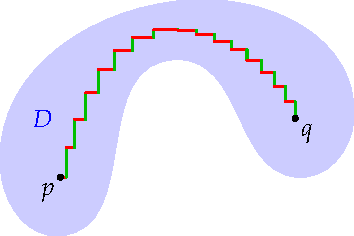
\includegraphics[scale=0.95]{analytic-topology}\vspace{-10pt}
	\end{minipage}\par
	\[
		\frac{u(x_2,y)-u(x_1,y)}{x_2-x_1}=u_x(\widehat x,y)
		\quad\text{and}\quad
		\frac{v(x_2,y)-v(x_1,y)}{x_2-x_1}=v_x(\widetilde x,y)
	\]
	By assumption $f'(z)=u_x+iv_x=0$, whence both partial derivatives are everywhere zero.
	It follows that $f(z)=u+iv$ takes the same value at both endpoints of any \textcolor{red}{horizontal segment}.\smallbreak
	The same holds along at the endpoints of any \textcolor{Green}{vertical segment}; this time we utilize $u_y=v_y=0$.\smallbreak
	By stepping along the segments in this fashion, we conclude that $f(q)=f(p)$. Since $p,q$ were arbitrary, $f$ is constant on $D$.
\end{proof}


\begin{cor}{}{modimpliesconst}
	If $f(z)$ is holomorphic with constant modulus $k=\nm{f(z)}$, then $f(z)$ is constant. 
\end{cor}

This is essentially trivial in the real case---think about why! The complex case needs a proof.

\begin{proof}
	Plainly $k^2=\nm{f(z)}^2=f(z)\cl{f(z)}$ is constant. If $k=0$, we are done. Otherwise, $\cl{f(z)}=\frac{k^2}{f(z)}$ is holomorphic (quotient rule!). Write $f(z)=u+iv$, whence $\cl{f(z)}=u-iv$, and consider the Cauchy--Riemann equations for \emph{both}:
	\[
		u_x=v_y,\qquad u_y=-v_x,\qquad u_x=-v_y,\qquad u_y=v_x
	\]
	All partial derivatives are therefore zero: $f'(z)=0$ and so $f$ is constant.
\end{proof}

The next result is worth stating now, since it provides a significant contrast with the real case. We'll prove it later once we've developed contour integration.

\begin{thm}{}{holoinfdiff}
	If $f(z)=u+iv$ is holomorphic, then $f$ is \emph{\bfseries infinitely differentiable.} Otherwise said:
	\begin{itemize}
	  \item $f^{(n)}(z)$ exists and is continuous for all $n\in\N$.
	  \item $u$ and $v$ have continuous partial derivatives of all orders.
	\end{itemize} 
\end{thm}

In real analysis, functions which are everywhere differentiable need not even be \emph{twice} differentiable, let alone infinitely so (Exercise \ref{exs:realoncediff}).


\boldinline{Harmonic Functions}

The \emph{second} partial derivatives of a holomorphic function satisfy a famous partial differential equation:
\[
	u_{xx}=\partials xu_x\overset{CR1}{=}\partials xv_y =v_{yx}\overset{(\ast)}{=}v_{xy}=\partials yv_x\overset{CR2}{=}-\partials yu_y=-u_{yy}
\]
Equality of the mixed partial derivatives $(\ast)$ follows because all derivatives are continuous (Theorem \ref{thm:holoinfdiff} and Clairaut's Theorem). The same equation holds for $v$. We conclude:

\begin{cor}{}{}
	If $f=u+iv$ is holomorphic, then $u$ and $v$ are \emph{harmonic functions}; solutions to \emph{Laplace's equation}
	\[
		\nabla^2u=u_{xx}+u_{yy}=0
	\]
\end{cor}

Laplace's equation is one of the most widely applied PDEs in mathematics and physics.

\begin{example}{}{}
	$f(z)=\frac 1z=\frac{x-iy}{x^2+y^2}$ is holomorphic on $\C\setminus\{0\}$; its real and imaginary parts are therefore harmonic away from the origin. Indeed,
	\begin{align*}
		u_{xx}+u_{yy}&=\left(\partials[^2]{x^2}+\partials[^2]{y^2}\right)\frac x{x^2+y^2}
		=\partials x\frac{y^2-x^2}{(x^2+y^2)^2}-\partials y\frac{2xy}{(x^2+y^2)^2}\\
		&=\frac{-2x(x^2+y^2)-4x(y^2-x^2)}{(x^2+y^2)^3}-\frac{2x(x^2+y^2)-8xy^2}{(x^2+y^2)^3}
		=0
	\end{align*}
\end{example}
\goodbreak

\boldinline{Analytic Continuations}

We finish this introduction to holomorphic functions with another surprising result whose proof will have to wait (this time for the theory of residues).

\begin{thm}[lower separated=false, sidebyside, sidebyside align=top seam, sidebyside gap=0pt, righthand width=0.38\linewidth]{}{analyticcont}
	Suppose $f$ and $g$ are holomorphic functions on an open connected domain $E$ and assume that \textcolor{red}{$f(z)=g(z)$} on some \textcolor{red}{path} contained in $E$.\smallbreak
	Then \textcolor{blue}{$f(z)=g(z)$} throughout $E$.
	\tcblower
	\flushright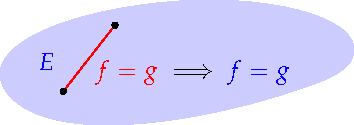
\includegraphics{analytic-topology2}
\end{thm}

This is highly counter-intuitive; you need only know the values of a holomorphic function on a tiny path to know the full function on its whole (connected) domain! This leads to a new concept.

\begin{defn}[lower separated=false, sidebyside, sidebyside align=top seam, sidebyside gap=0pt, righthand width=0.38\linewidth]{}{}
	Let $D\subseteq E$ be open connected domains and $g:E\to \C$ holomorphic. Let $f:D\to\C$ be the restriction of $g$ to $D$; that is $f(z)=g(z)$ on $D$.\smallbreak
	We call $g$ the \emph{analytic continuation} of $f$ to $E$.\tcblower
	\flushright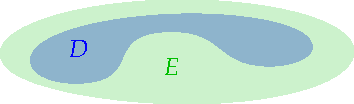
\includegraphics{analytic-topology3}
\end{defn}

By Theorem \ref{thm:analyticcont}, the analytic continuation of $f$ to $E$ is unique. There are, however, some subtleties, which we explore a little in the next example:
\begin{itemize}\itemsep2pt
  \item Given $f$ analytic on $D$, an analytic continuation to $E\supseteq D$ is not guaranteed to exist.
  \item The choice of extended domain $E$ \emph{really} matters.
\end{itemize}

\begin{example}{}{sqrtzanalcont}
	Let $f(z)=\sqrt z=\sqrt r\polar{i\theta}2$ be the principal square root whose domain $D$ is the \textcolor{Green}{first quadrant}. Exercise \ref{exs:sqrtzdiff} verifies that $f$ is holomorphic on $D$.\par
	The pictures describe \emph{two} analytic continuations of $f$: in both cases the point $w=\polarn{3\pi i}4=\polar{5\pi i}4$ is used for comparison.\par
	\begin{minipage}[t]{0.61\linewidth}\vspace{-5pt}
		\begin{enumerate}
		  \item Let $G$ be the \textcolor{blue}{plane omitting the non-positive real axis} and define
			\[
				g:G\to\C:z\mapsto \sqrt r\polar{i\theta}2,\quad \theta=\Arg z\in(-\pi,\pi)
			\]
			The codomain of $g$ is the \textcolor{blue}{right half-plane}. Observe that $g(w)=\polarn{3\pi i}8$ lies in the \emph{fourth quadrant.}
			\item	Let $H$ be the \textcolor{orange}{plane omitting the non-positive imaginary axis} and define
			\[
				h:H\to\C:z\mapsto \sqrt r\polar{i\theta}2,\quad \theta=\arg z\in(-\tfrac\pi 2,\tfrac{3\pi}2)
			\]
			The codomain of $h$ is the \textcolor{orange}{upper-right half-plane}. Moreover $h(w)=\polar{5\pi i}8=-g(w)$ lies in the \emph{second quadrant.}
		\end{enumerate}
	\end{minipage}
	\hfill
	\begin{minipage}[t]{0.38\linewidth}\vspace{-15pt}
		\flushright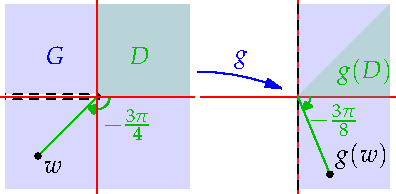
\includegraphics[scale=0.95]{analytic-cont1}\\
		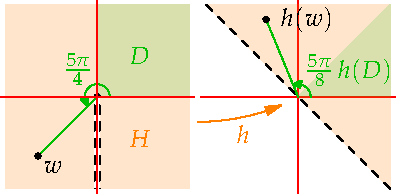
\includegraphics[scale=0.95]{analytic-cont2}
	\end{minipage}
	\medbreak
	The two analytic continuations of $f$ disagree on the intersection of their domains!\smallbreak
	In fact the omissions chosen for $G,H$ are necessary: there is no analytic continuation of $f$ to the punctured plane $\C\setminus\{0\}$, or indeed to any domain in which it is possible to loop completely around the origin. We shall return to this topic in Chapter \ref{chap:functions}\ldots
\end{example}

\goodbreak



\begin{exercises}{}
	\exstart Suppose $g'(z)=h'(z)$  on an open connected domain $D$. Prove that $h(z)=g(z)+c$ for some constant $c\in\C$.\vspace{-5pt}
	\begin{enumerate}\setcounter{enumi}{1}
	  \item[]\emph{Equivalently: if $g(z)$ and $h(z)$ are anti-derivatives of $f(z)$, then $g(z)-h(z)$ is constant}
	  
	  
	  \item Verify that $u=e^{nx}\cos ny$ and $v=e^{nx}\sin ny$ are harmonic functions for any $n\in\Z$.
	  
	  
	  \item Prove or disprove: if $u,v:D\to\R$ are harmonic functions on an open set $D\subseteq\R^2$, then $f(z):=u(x,y)+iv(x,y)$ is holomorphic.
	  
	  
	  \item\label{exs:realoncediff} Define $f:\R\to\R$ by
		\[
			f(x)=x\nm x=
			\begin{cases}
				x^2&\text{if }x\ge 0\\
				-x^2&\text{if }x<0
			\end{cases}
		\]
		Show that $f$ is differentiable, but not \emph{twice} so (\emph{an impossible property for complex functions}).

	  
	  \item\label{exs:crpolar} Suppose $f(z)=u+iv$ and write $z=x+iy=re^{i\theta}$ in polar form.
	  \begin{enumerate}
	    \item Use the chain rule applied to the polar co-ordinate relations $x=r\cos\theta$, $y=r\sin\theta$ to compute the partial derivatives $u_r,u_\theta,v_r,v_\theta$ in terms of $u_x,u_y,v_x,v_y$.
	    
	  	\item Deduce the polar form of the Cauchy--Riemann equations:
			\[
				ru_r=v_\theta\qquad u_\theta=-rv_r,\qquad f'(z)=e^{-i\theta}(u_r+iv_r) =\frac{-i}{z}(u_\theta+iv_\theta)
			\]
		\end{enumerate}
		
		
		\item Prove the polar form of Laplace's equation:
		\[
			r^2u_{rr}+ru_r+u_{\theta\theta}=0
		\]
			
			
		\item Show that $u=r^n\cos n\theta$ is a harmonic function for any $n\in\N$: find \emph{two} ways to show that this is true!
		
		
		\item Suppose $f:\C\to\C$ is an entire function such that $f(iy)=-iy^3$ whenever $z=iy$ lies on the imaginary axis. What is the value $f(2)$? Explain your answer.\par
		(\emph{Hint: Think about analytic continuations})
		
		
		\item The function $f(z)=\frac 1z$ is holomorphic on $\C\setminus\{0\}$. Explain why there is no analytic continuation of $f$ that is holomorphic at $z=0$.
		
		
		\item\label{exs:sqrtzdiff}
		\begin{enumerate}
		  \item Use Exercise \ref{exs:crpolar} to prove that $f(z)=\sqrt z=\sqrt r\polar{i\theta}2$ is holomorphic on the first quadrant and find $f'(z)$. Moreover, explain why the functions $g,h$ in Example \ref{ex:sqrtzanalcont} are holomorphic and therefore both analytic continuations of $f$.
		  
		  \item Prove that there exists no analytic continuation of $g$ to any set larger than $G$.\par
			(\emph{Hint: suppose the extended domain contains $-r\in\R^-$. Now use the fact that an analytic continuation must be continuous at $-r\ldots$})
		\end{enumerate}
	\end{enumerate}
\end{exercises}